%!TEX root = ../thesis.tex

\section{学習フェーズ}
提案手法で用いる学習フェーズを\figref{Fig:suggest_learning_sys}に示す. 経路追従行動を行う地図ベースの制御器から目標方向を生成し, データセットに加えている. 提案手法では, \figref{Fig:overview}に示すようにLiDARとオドメトリを入力とする地図ベースの制御器による経路追従行動を, カメラ画像と目標方向を用いて模倣学習する.

\begin{figure}[hbtp]
  \centering
 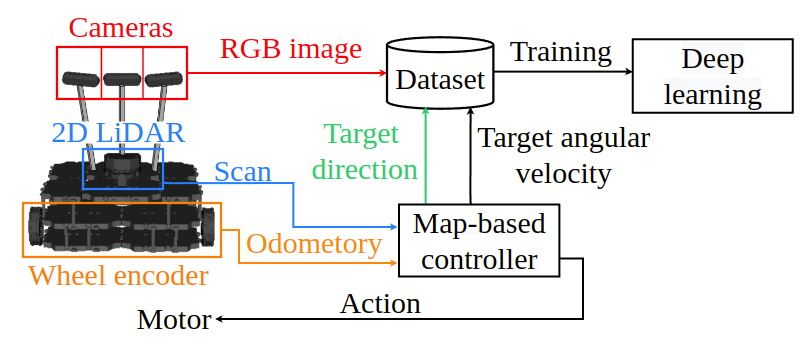
\includegraphics[keepaspectratio, scale=0.45]
      {images/suggest_learning_sys.png}
 \caption{Learning phase system of proposed method}
 \label{Fig:suggest_learning_sys}
\end{figure}

\begin{figure}[hbtp]
  \centering
 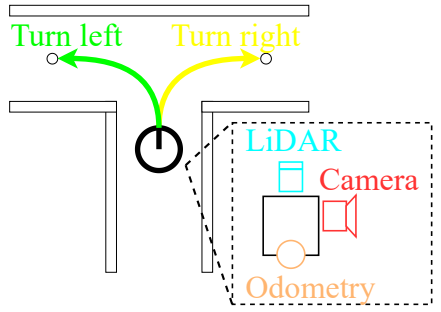
\includegraphics[keepaspectratio, scale=0.6]
      {images/overview.png}
 \caption{Overview learning phase}
 \label{Fig:overview}
\end{figure}

% \subsubsection{etc...}
\newpage
